\documentclass[letterpaper]{article}
\usepackage{amssymb}
\usepackage{amsmath}
\usepackage{graphicx}
\usepackage{listings}
\usepackage{bbm}
\usepackage[colorlinks]{hyperref}

\usepackage{tikz}
\usepackage{tikzsymbols}

\usepackage{color} %red, green, blue, yellow, cyan, magenta, black, white
\usepackage{empheq}
\definecolor{fakeblue}{rgb}{0.9, 0.9, 1}

\usepackage[final]{nips_2016}

\begin{document}

\title{10-703: Deep RL and Controls Homework 2}
\author{Adithya Murali \& Alexander Spitzer}

\date{\vspace{-5ex}}

\maketitle

\section{Questions}
The tabular Q-learning update is shown below.
\begin{equation}
  Q(s, a) := Q(s, a) + \alpha\left(r + \gamma \max_{a' \in A} Q(s', a') - Q(s, a)\right)
\end{equation}

In the function approximation setting, the weight update is below.
\begin{equation}
  w := w + \alpha\left(r + \gamma \max_{a' \in A} Q_w(s', a') - Q_w(s, a)\right) \nabla_wQ_w(s, a)
\end{equation}

To see that the function approximation setting is a generalization of the tabular setting, assume that $Q_w(s, a) = w^\top\phi(s, a)$ and $\phi(s, a) = \phi(s, a)_{s',a'} = \mathbbm{1}[s' = s, a' = a]$.

Note that $\nabla_wQ_w(s, a) = \phi(s, a)$.

Now, write down the Q-learning update for the function approximation setting using the weight update shown above.
\begin{align}
  Q_w(s, a) = w^\top\phi(s, a) &:= \left(w + \alpha\left(r + \gamma \max_{a' \in A} Q_w(s', a') - Q_w(s, a)\right) \nabla_wQ_w(s, a)\right)^\top\phi(s, a)\nonumber\\
  &:= Q_w(s, a) + \left(\alpha\left(r + \gamma \max_{a' \in A} Q_w(s', a') - Q_w(s, a)\right)\phi(s, a)\right)^\top\phi(s, a)\nonumber\\
  &:= Q_w(s, a) + \alpha\left(r + \gamma \max_{a' \in A} Q_w(s', a') - Q_w(s, a)\right)\phi(s, a)^\top\phi(s, a)\nonumber\\
  &:= Q_w(s, a) + \alpha\left(r + \gamma \max_{a' \in A} Q_w(s', a') - Q_w(s, a)\right)
\end{align}

The last step holds because $\phi(s, a) $ is equal to one for only one state action pair and zero for all others.

We see that the Q-learning update dervied is equal to that of the tabular setting.

\section{Implementation}

Our algorithm is implemented entirely in Python using Tensorflow (no Keras) and we mainly follow the details and hyperparameters provided in the DQN Nature paper.
\subsection{Preprocessing}
The incoming frames of size 210 x 160 x 3 are converted to grayscale using the Python Imaging Library and resized to a size of 84 x 84 before each forward pass. Because cropping the image to a square size might cut off important areas of the game screen, we instead resize the entire image to the desired size. This has the drawback of squeezing the entire game view by a constant factor, but we found that to be inconsequential.

Although the original image frame pixel intensities vary between 0 and 255, we convert pixel values to floats with values between 0 and 1 before feeding any images to the network. This is desirable because it keeps the network's input data distribution closer to standard normal, which has shown to improve training performance. If all the input values are much greater than zero, it is likely that the input to the nonlinear layer will be in a very linear region, either far from the nonlinearity if the rectifier is used, or where the gradients are small if sigmoid or tanh are used.

	In some games (notably SpaceInvaders) there is a "flickering" effect where the bullets will disappear in alternating frames. Training with this flickering might confuse the agent about the environment's dynamics. To overcome this problem, we take the maximum value of each pixel between the grayscale current frame and the previous one to be the grayscale frame used by the network.

\subsection{Details}

\begin{enumerate}
  \item \textbf{Frame skipping:} We use the fully deterministic environments provided by OpenAI's Atari Gym. These environments always skip a fixed number of frames (as described in the DeepMind papers). The actions for the skipped frames are the chosen to be that of the previous action selected.
  \item \textbf{Episode guidance:} We treat the loss of life by the agent as an episode ending event. This compels the agent to stay alive for as long as possible, though it is questionable if that is indeed always the best option. In some games, it may be advantageous to die to get out of a sticky situation.
  \item \textbf{Training:} We use the huber loss recommended in the code template and RMSProp as the optimizer.
\end{enumerate}

\subsection{Models}
We implement three different Q network architectures: a simple linear network, the original deep Q network, and the dueling Q network. Our models take as input a sequence of four of the last game frames seen. The matrix parameters of our models are all initialized using Xavier initialization, while the bias terms are initialized to 0. All nonlinearities are rectifier units.

All of our models can be optionally trained using the Double DQN algorithm.
\subsubsection{Linear Q Network}
The linear Q network has one linear layer with an affine bias term. The output is, like the other Q networks, a Q value for every action.
\subsubsection{Deep Q Network}
The DQN has 2 convolutional layers. The first consists of 16 8 x 8 filters with a stride of 4 and the second consists of 32 4 x 4 filters with a stride of 2. This is followed by a fully connected layer with 256 hidden units and finally a linear output layer.
\subsubsection{Dueling Q Network}
The dueling DQN has the same convolutional layers as the DQN. However, the output of the last convolutional layer is split into two streams, each of which has a hidden layer of 256 hidden units and a linear output layer. The two streams are then recombined as in the Dueling DQN paper.


\subsection{Hyperparameters}
\begin{center}
  \begin{tabular}{|l|l|p{9cm}|}
    \hline
    \textbf{Parameter} & \textbf{Value} & \textbf{Description} \\ \hline
    $\gamma$ & 0.99 & Reward discount \\ \hline
    Learning rate & 0.00025 & Learning rate used by RMSProp \\ \hline
    $\epsilon$ & 0.10 & Final epsilon used for $\epsilon$-greedy \\ \hline
    Momemtum & 0.95 & Momenmtum used by RMSProp \\ \hline
    Minimum squared gradient & 0.01 & Constant added to squared gradient in denominator of RMSProp update \\ \hline
    Exploration Decay Iterations & 1000000 & Number of iterations taken for $\epsilon$ to decay from 1.0 to 0.10 \\ \hline
    Training frequency & 4 & Number of actions taken before every network update \\ \hline
    Window size & 4 & Number of consective frames used as network input \\ \hline
    Replay memory size & $10^6$ & Maximum number of transitions held in the replay memory \\ \hline
    Target network update frequency & 10000 & Number of online network updates before copying parameters to the target network \\ \hline
    Batch size & 32 & Size of minibatch used in Stochastic Gradient Descent \\ \hline
    Exploration Iterations & 50000 & Number of experiences collected before any training is done \\\hline
  \end{tabular}
\end{center}
\section{Results}

All of our experiments are run on the game SpaceInvaders, using the \texttt{SpaceInvadersDeterministic-v3} Atari gym environment. As described above, this environment is deterministic and only reports every $3^{\text{rd}}$ frame. The actions taken for skipped frames are equal to that given on the previously reported frame.

We compare 6 different approaches: a linear Q network without experience replay and without target fixing, a linear Q network, a linear double Q network, the Deep Q Network, the double Deep Q Network, and the dueling Deep Q Network.

We train for 2 million iterations. We evaluate the performance of our network every 10,000 training iterations. Since we train on deterministic environments, the reward is the same for any given network, and thus we run one episode per evaluation. Performance plots during training for all 6 approaches are shown below.

\begin{center}
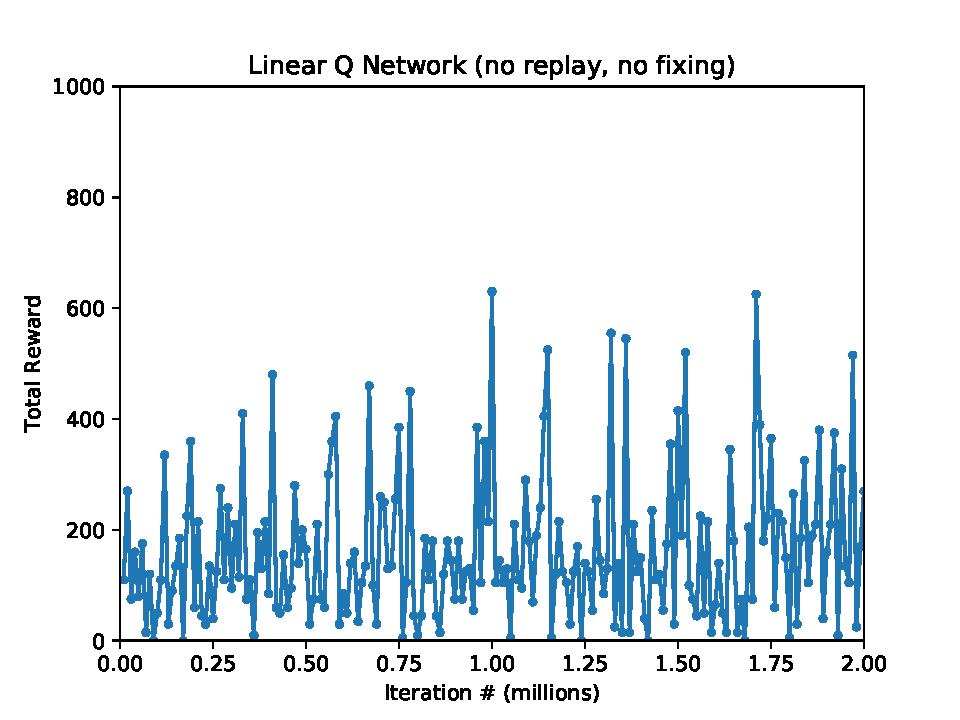
\includegraphics[width=6.8cm]{../figs/reward_lqn_nomem.pdf}
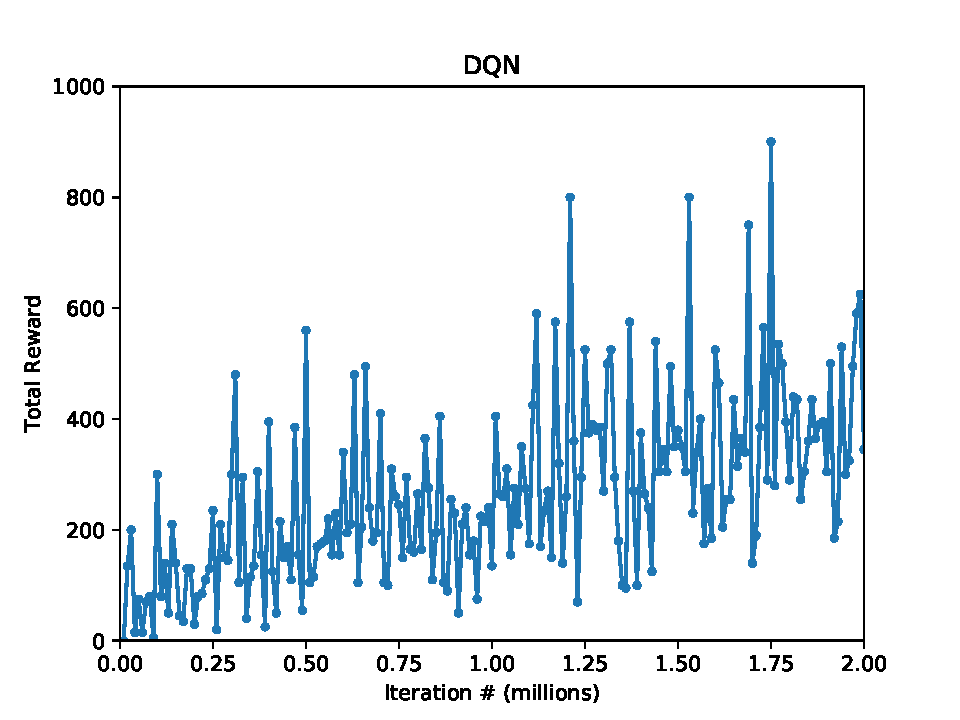
\includegraphics[width=6.8cm]{../figs/reward_dqn.pdf}
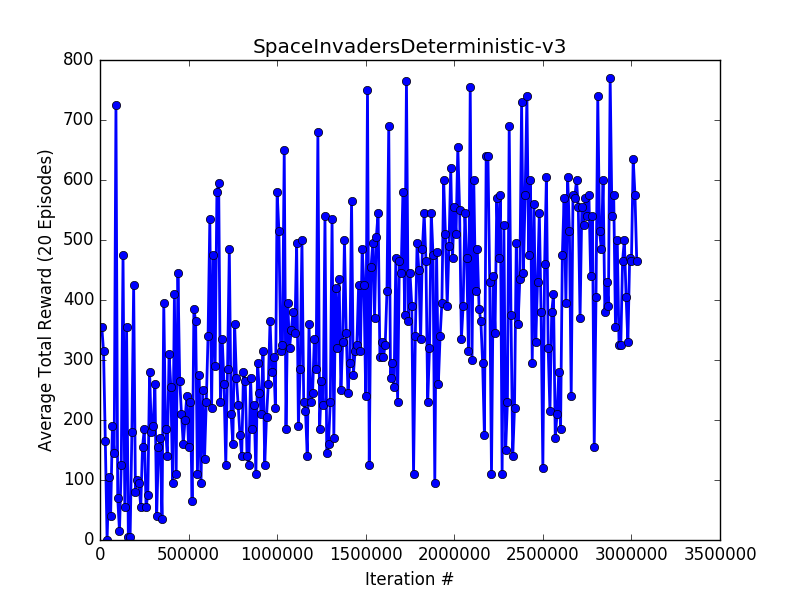
\includegraphics[width=6.8cm]{../figs/DQN_double.png}
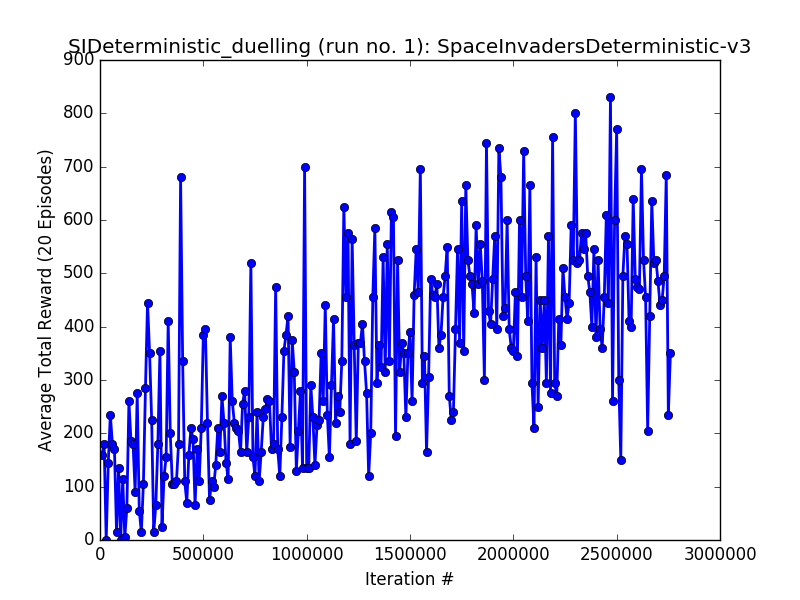
\includegraphics[width=6.8cm]{../figs/DQN_duelling.png}
\end{center}

\begin{table}[!ht]
\centering
\label{results}
\begin{tabular}{|l|l|l|}
\hline
                                  & \multicolumn{2}{c|}{Environment} \\ \hline
Model                       & Deterministic & Stochastic \\ \hline
Linear (No memory, target fixing) &  420.0             &  189.75 $\pm$ 109.93          \\ \hline
Linear Q Network                  &  135.0             &  161.95 $\pm$ 72.849          \\ \hline
Linear Double Q Network           &  5.0             &  10 $\pm$ 5.431         \\ \hline
DQN                               &  460.0             & 493.45 $\pm$ 141.12     \\ \hline
Double DQN                        &  570.0            &  497.9 $\pm$ 161.49          \\ \hline
Duelling DQN                      &  470.0             & 435.5 $\pm$ 161.96  \\ \hline
\end{tabular}

\caption{Average total reward results for SpaceInvaders. The deterministic environment is \texttt{SpaceInvadersDeterministic-v3} and the stochastic environment is \texttt{SpaceInvaders-v3}.}
\end{table}
See Table 1 for the average total reward results of all of our models after full training. We see that the Deep Q Networks handily outperformed the linear networks, with Double DQN and regular DQN slightly outperforming Dueling DQN. We note that due to the high standard deviation of the rewards on the stochastic environment, and the large variance of the reward in time during training, we should not place too much emphasis on the particular deterministic reward. For example, the basic linear Q network without experience replay and without target fixing did quite well on the deterministic environment, but that was just luck; stochastic performance is about the same as the other linear networks.

Videos of our agent's performance are available as supplementary material in the code submission zip. The Deep Q Networks learn effective strategies such as dodging bullets and hiding behind structures. In addition, the purple flying saucer is shot almost every time it appears, possibly indicating that the agent has learned to time its bullets to intercept the bonus.

\end{document}
